\documentclass[11pt, dvipsnames, handout]{beamer}
\newtoggle{full}
\settoggle{full}{true}

\newtoggle{covered}
\settoggle{covered}{false}

\newtoggle{presentable}
\settoggle{presentable}{false}

\newtoggle{dualscreen}
\settoggle{dualscreen}{false}

\usepackage{pgfplots}
%\pgfplotsset{compat = newest}

\usepackage{pgfpages}

\setbeamertemplate{note page}{\pagecolor{yellow!5}\vfill \insertnote \vfill}
\usepackage{collect}
\definecollection{notes}
\newcounter{notestaken}

\usepackage{xpatch}

\usepackage{ulem}

\usepackage[framemethod=tikz]{mdframed}

\usepackage{scalerel}
\usepackage{calc}

%\usepackage{enumitem}
\setlength\fboxsep{.2em}

\usepackage{graphicx} % Allows including images
\usepackage{booktabs} % Allows the use of \toprule, \midrule and \bottomrule in tables

\xpatchcmd{\itemize}
  {\def\makelabel}
  {\setlength{\itemsep}{0.65 em}\def\makelabel}
  {}
  {}


\xpatchcmd{\beamer@enum@}
  {\def\makelabel}
  {\setlength{\itemsep}{0.65 em}\def\makelabel}
  {}
  {}


%\makeatletter
%\renewcommand{\itemize}[1][]{%
%  \beamer@ifempty{#1}{}{\def\beamer@defaultospec{#1}}%
%  \ifnum \@itemdepth >2\relax\@toodeep\else
%    \advance\@itemdepth\@ne
%    \beamer@computepref\@itemdepth% sets \beameritemnestingprefix
%    \usebeamerfont{itemize/enumerate \beameritemnestingprefix body}%
%    \usebeamercolor[fg]{itemize/enumerate \beameritemnestingprefix body}%
%    \usebeamertemplate{itemize/enumerate \beameritemnestingprefix body begin}%
%    \list
%      {\usebeamertemplate{itemize \beameritemnestingprefix item}}
%      {%
%        \setlength\topsep{1em}%NEW
%        \setlength\partopsep{1em}%NEW
%        \setlength\itemsep{1em}%NEW
%        \def\makelabel##1{%
%          {%
%            \hss\llap{{%
%                \usebeamerfont*{itemize \beameritemnestingprefix item}%
%                \usebeamercolor[fg]{itemize \beameritemnestingprefix item}##1}}%
%          }%
%        }%
%      }
%  \fi%
%  \beamer@cramped%
%  \raggedright%
%  \beamer@firstlineitemizeunskip%
%}
%
%
%
%
%
%\makeatother

%\setlist[beamer@enum@]{topsep=1 em}
%\let\origcheckmark\checkmark %screw you dingbat
%\let\checkmark\undefined %screw you dingbat
%\usepackage{dingbat} 
%\let\checkmark\origcheckmark %screw you dingbat






%\usepackage{fontawesome}

\usepackage{mathtools}
\usepackage{etoolbox, calculator}

\usepackage{xcolor}
\usepackage{tikz}
\usetikzlibrary{arrows.meta}
\usetikzlibrary{calc}
\usepackage[nomessages]{fp}
\usepackage{transparent}
\usepackage{accsupp}
%\usepackage{color, xcolor}

%colorblind-friendly palette
%\definecolor{dblue}{RGB}{51,34,136}
\definecolor{lblue}{RGB}{136,204,238}
%\definecolor{green}{RGB}{17,119,51}
\definecolor{tan}{RGB}{221,204,119}
%\definecolor{mauve}{RGB}{204,102,119}

\usepackage{tcolorbox}



\usepackage{xifthen}
\usepackage{nicefrac}
\usepackage{amsmath}
\usepackage{amsthm}
\usepackage{amssymb}
\theoremstyle{definition}
\newtheorem*{define}{Definition}
\newtheorem*{recall}{Recall}


\DeclareMathOperator{\tr}{tr}

\usepackage{multicol}
%\setlength{\columnsep}{1cm}

\usepackage{tablists, amsmath,vwcol, cancel, polynom}
\usetikzlibrary{shapes, patterns, decorations.shapes}
%\usepackage{tikzpeople}
\tikzstyle{vertex}=[shape=circle, minimum size=2mm, inner sep=0, fill]
\tikzstyle{opendot}=[shape=circle, minimum size=2mm, inner sep=0, fill=white, draw]

% common math quick commands
\newcommand{\nicedd}[2]{\nicefrac{\text{d}#1}{\text{d}#2}}
\newcommand{\dd}[2]{\dfrac{\text{d}#1}{\text{d}#2}}
\newcommand{\pd}[2]{\dfrac{\partial #1}{\partial#2}}
\renewcommand{\d}[1]{\text{d}#1}
\newcommand{\ddn}[3]{\dfrac{\text{d}^{#3}#1}{\text{d}#2^{#3}}}
\newcommand{\pdn}[3]{\dfrac{\partial^{#3}#1}{\partial#2^{#3}}}
\newcommand{\p}[0]{^{\prime}}
\newcommand{\pp}[0]{^{\prime\prime}}
\newcommand{\op}[2][\text{L}]{#1 \left[ #2 \right]}

\newcommand{\lap}[1]{\mathcal{L}\left\{#1\right\}}
\newcommand{\lapinv}[1]{\mathcal{L}^{-1}\left\{#1\right\}}
\newcommand{\lapint}[1]{\int_0^\infty e^{-st}#1dt}
\newcommand{\evalat}[2]{\Big|_{#1}^{#2}}

\newcommand{\paren}[1]{ \left( #1 \right)}

\newcommand{\haxis}[4][\normcolor]{\draw[#1, <->] (-#2,0)--(#3,0) node[right]{$#4$}; }

\newcommand{\circled}[1]{\raisebox{.5pt}{\textcircled{\raisebox{-.9pt} {#1}}}}
\newcommand{\axis}[4]{\draw[\normcolor, <->] (-#1,0)--(#2,0) 
node[right]{$x$};
\draw[help lines, <->] (0,-#3)--(0,#4) node[above]{$y$};}

\newcommand{\laxis}[6]{\draw[<->] (-#1,0)--(#2,0) 
node[right]{$#5$};
\draw[ <->] (0,-#3)--(0,#4) node[above]{$#6$};}
\newcommand{\xcoord}[2]{
	\draw (#1,.2)--(#1,-.2) node[below]{$#2$};}
\newcommand{\textnode}[3]{
	\draw (#1,#2) node[below]{$#3$};}
	
\newcommand{\nxcoord}[2]{
	\draw (#1,-.2)--(#1,.2) node[above]{$#2$};}
\newcommand{\ycoord}[2]{
	\draw (.2,#1)--(-.2,#1) node[left]{$#2$};}
\newcommand{\nycoord}[2]{
	\draw (-.2,#1)--(.2,#1) node[right]{$#2$};}
\newcommand{\dlim}{\displaystyle\lim}
\newcommand{\dlimx}[1]{\displaystyle\lim_{x \rightarrow #1}}
\newcommand{\stickfig}[2]{
	\draw (#1,#2) arc(-90:270:2mm);
	\draw (#1,#2)--(#1,#2-.5) (#1-.25,#2-.75)--(#1,#2-.5)--(#1+.25,#2-.75) (#1-.2,#2-.2)--(#1+.2,#2-.2);}	

%\newcounter{example}
%\setcounter{example}{1}
%\newcounter{preFrameExample}
%\AtBeginEnvironment{frame}{\setcounter{preFrameExample}{\value{example}}}
%\newcommand{\ex}[1]{
%	 \setcounter{example}{\value{preFrameExample}}
%	 \textcolor{green}{\small\fbox{Example \arabic{example}: #1}}\\[8pt]
%	\stepcounter{example}}
%\newcommand{\exans}[1]{
%	\SUBTRACT{\value{preFrameExample}}{1}{\n}
%	 \textcolor{green}{\small\fbox{Solution \n: #1}}\\[8pt]}
\mode<presentation> {

% The Beamer class comes with a number of default slide themes
% which change the colors and layouts of slides. Below this is a list
% of all the themes, uncomment each in turn to see what they look like.


\usetheme{CambridgeUS}
\usecolortheme[named=black]{structure}


\newcommand{\studentcolor}[0]{ForestGreen}
\newcommand{\normcolor}[0]{NavyBlue}
\newcommand{\alertcolor}{Red}

\setbeamercolor{normal text}{fg=\normcolor}
\setbeamercolor{frametitle}{fg=\normcolor}
\setbeamercolor{section in head/foot}{fg=Black, bg=Gray!20}
\setbeamercolor{subsection in head/foot}{fg=Green!70!Black, bg=Gray!10}
\setbeamercolor{alerted text}{fg=\alertcolor}
\setbeamerfont{alerted text}{series=\bf}
\setbeamertemplate{enumerate items}[default]
\setbeamercolor{enumerate item}{fg=\normcolor}

\setbeamertemplate{footline} % To remove the footer line in all slides uncomment this line
%\setbeamertemplate{footline}[page number] % To replace the footer line in all slides with a simple slide count uncomment this line

\setbeamertemplate{navigation symbols}{} % To remove the navigation symbols from the bottom of all slides uncomment this line
}

\newcommand{\alertbox}[1]{\tcbox[on line, colframe=\alertcolor, colback=White, left=2pt,right=2pt,top=2pt,bottom=2pt]{\usebeamercolor*{normal text}#1}}


\newcommand{\startstu}{\setbeamercolor{normal text}{fg=\studentcolor}\usebeamercolor*{normal text}\setbeamercolor{enumerate item}{fg=\studentcolor}\usebeamercolor*{enumerate item}}
\newcommand{\stopstu}{\setbeamercolor{normal text}{fg=\normcolor}\usebeamercolor*{normal text}\setbeamercolor{enumerate item}{fg=\normcolor}\usebeamercolor*{enumerate item}}

\newcommand{\takenote}[1]{ \begin{collect}{notes}{}{}{}{}  #1  \end{collect}  \addtocounter{notestaken}{1}} %\ifthenelse{\value{notestaken}>0}{\hrulefill\\}{}

\makeatletter
\newcommand{\cover}{\alt{\beamer@makecovered}{\beamer@fakeinvisible}}
\newcommand{\ucover}[1]{\iftoggle{full}{}{\beamer@endcovered} \stopstu #1\startstu \iftoggle{full}{}{\beamer@startcovered} }
%\newcommand{\ucover}[1]{\beamer@endcovered \stopstu #1\startstu \beamer@startcovered }
\makeatother

\newcommand{\skippause}{ \addtocounter{beamerpauses}{-1}}
\newcommand{\blockpres}{ \skippause \pause }

\newcommand{\studentify}[1]{\startstu #1  \stopstu }
\newcommand{\student}[1]{\iftoggle{full}{ \pause  \studentify{#1} }{\iftoggle{covered}{\studentify{#1}}{\cover{  #1 }}}}
\newcommand{\cstudent}[1]{\student{\begin{center} #1 \end{center}}}
\newcommand{\fullonly}[1]{\iftoggle{full}{ #1}{}}
\newcommand{\presentonly}[1]{\iftoggle{presentable}{ #1}{}}

\usepackage{xparse}
\usepackage{xifthen}

% shortcuts for commonly-used presentation elements
%\NewDocumentCommand{\slide}{o m}
% {\IfValueTF{#1}{\begin{frame}[t]{#1}}{\begin{frame}[t]} #2 \end{frame}}

\newtoggle{iscovered}

\newcommand{\slide}[2][]{%
%\setcounter{notestaken}{0}
\takenote{#2} 
%\ifthenelse{\equal{#1}{}}{\begin{frame}[t]}{\begin{frame}[t]{#1}} #2 \ifthenelse{\value{notestaken}>0}{ \note{\includecollection{notes}}}{} \end{frame}%
\ifthenelse{\equal{#1}{}}{\begin{frame}[t]}{\begin{frame}[t]{#1}} #2 \iftoggle{covered}{\settoggle{iscovered}{true}}{\settoggle{iscovered}{false}}  \note{ \iftoggle{iscovered}{}{\settoggle{covered}{true}} #2 \iftoggle{iscovered}{}{\settoggle{covered}{false}} } \end{frame}%
%\setcounter{notestaken}{0}
}
\newcommand{\defn}[2][]{%
 \setcounter{listcounter}{0}%
\ifthenelse{\equal{#1}{}}{\begin{block}{Definition}}{\begin{block}{#1 :}}%
 #2 \vspace{0.25em} \ifthenelse{\value{listcounter}>0}{\skippause}{} \pause \end{block}%
}



\newcommand{\arr}[2]{\begin{array}{#1}#2\end{array}}
\newcommand{\mat}[2]{\left[\arr{#1}{#2}\right]}
\newcommand{\carray}[1]{\arr{c}{#1}}
\newcommand{\larray}[1]{\arr{l}{#1}}
\newcommand{\rarray}[1]{\arr{r}{#1}}
\newcommand{\colvec}[1]{\mat{c}{#1}}

\newcommand{\itmz}[1]{\addtocounter{listcounter}{1} \begin{itemize}#1 \end{itemize} }
\newcommand{\subitem}[1]{\addtocounter{listcounter}{1} \begin{itemize} \item #1 \end{itemize}}
%
\newcommand{\enum}[1]{\addtocounter{listcounter}{1} \begin{enumerate} #1  \end{enumerate}  }


\newcommand{\algnlbl}[1]{\begin{align}#1  \end{align}} 
\newcommand{\algn}[1]{\begin{align*}#1  \end{align*}} 
\newcommand{\lgn}[1]{ \action<+->{#1} }
\newcommand{\slgn}[1]{\iftoggle{full}{\action<+->{ \startstu #1 \stopstu}}{ \cover{ #1 } } \takenote{$#1$}}

\newcommand{\chckmrk}{\alert{\checkmark}}

\usepackage{pifont}
\newcommand{\xmark}{\alert{\text{\large \ding{55}}}}

\newcommand{\return}[0]{\raisebox{.5ex}{\rotatebox[origin=c]{180}{$\Lsh$}}}
\usepackage{pbox}
%\newcommand{\ex}[1]{\rotatebox[origin=c]{10}{\uline{ex}}:$\;$\pbox[t][][b]{0.9\linewidth}{#1}}
\newcommand{\ex}[1]{\uline{ex}:$\;$\pbox[t][][t]{0.9\linewidth}{#1}}
\newcommand{\eg}[1]{e.g.,$\;$\pbox[t][][t]{0.9\linewidth}{#1}}
\newcommand{\tikzplot}[8][]{%
\begin{tikzpicture}

\begin{scope}[]%
\clip(-#2,-#4) rectangle (#3,#5);%
#8%
\end{scope}%
\laxis{#2}{#3}{#4}{#5}{#6}{#7}%
#1
\end{tikzpicture}%
}


\newcommand{\cancelslide}[1]{%
\begingroup%
\setbeamertemplate{background canvas}{%
\begin{tikzpicture}[remember picture,overlay]%
\draw[line width=2pt,red!60!black] %
  (current page.north west) -- (current page.south east);%
\draw[line width=2pt,red!60!black] %
  (current page.south west) -- (current page.north east);%
\end{tikzpicture}}%
#1%
\endgroup%
}
\renewcommand{\CancelColor}{\color{red}}
\newcommand{\twocols}[3][0.5]{\begin{columns}\begin{column}{#1\textwidth}#2\end{column}\hspace{1em}\vrule{}\hspace{1em}\begin{column}{#1\textwidth}#3\end{column}\end{columns}}

\newcommand{\twomini}[5][1]{\calculatespace \begin{minipage}[t]{\columnwidth}\begin{minipage}[][#1\contentheight][t]{#2\columnwidth}#4\end{minipage}\hfill\begin{minipage}[][#1\contentheight][t]{#3\columnwidth}#5\end{minipage}\end{minipage}}

\newcommand{\threemini}[7][1]{\calculatespace \begin{minipage}[t]{\columnwidth}\begin{minipage}[][#1\contentheight][t]{#2\columnwidth}#5\end{minipage}\hfill\begin{minipage}[][#1\contentheight][t]{#4\columnwidth}#6\end{minipage}\hfill\begin{minipage}[][#1\contentheight][t]{#3\columnwidth}#7\end{minipage}\end{minipage}}


\newcounter{listcounter}
\setcounter{listcounter}{0}



\newif\ifsidebartheme
\sidebarthemetrue

\newdimen\contentheight
\newdimen\contentwidth
\newdimen\contentleft
\newdimen\contentbottom
\makeatletter
\newcommand*{\calculatespace}{%
\contentheight=\paperheight%
\ifx\beamer@frametitle\@empty%
    \setbox\@tempboxa=\box\voidb@x%
  \else%
    \setbox\@tempboxa=\vbox{%
      \vbox{}%
      {\parskip0pt\usebeamertemplate***{frametitle}}%
    }%
    \ifsidebartheme%
      \advance\contentheight by-1em%
    \fi%
  \fi%
\advance\contentheight by-\ht\@tempboxa%
\advance\contentheight by-\dp\@tempboxa%
\advance\contentheight by-\beamer@frametopskip%
\ifbeamer@plainframe%
\contentbottom=0pt%
\else%
\advance\contentheight by-\headheight%
\advance\contentheight by\headdp%
\advance\contentheight by-\footheight%
\advance\contentheight by4pt%
\contentbottom=\footheight%
\advance\contentbottom by-4pt%
\fi%
\contentwidth=\paperwidth%
\ifbeamer@plainframe%
\contentleft=0pt%
\else%
\advance\contentwidth by-\beamer@rightsidebar%
\advance\contentwidth by-\beamer@leftsidebar\relax%
\contentleft=\beamer@leftsidebar%
\fi%
}
\makeatother


\usetikzlibrary{arrows}
\iftoggle{dualscreen}{\setbeameroption{show notes on second screen=right}}{}


\begin{document}

\section{Lecture 14}
\subsection{Preamble}


\slide[Recall: $ay''+by'+cy=f(t)\quad \text{with } y(0)=y_0, y'(0)=v_0$]{\vspace{-1em}
\[
\Rightarrow Y(s) =\underbrace{ \frac{F(s)}{as^2+bs+c}}_{\text{particular part}}+ \underbrace{\frac{ay_0s+(by_0 +av_0)}{as^2+bs+c}}_{\text{homogeneous part}}
\]

\centerline{We now focus on cases where the forcing function $f(t)$ is not continuous.}

\vfill
Two types of such forcing:\vfill
\twomini[.3]{.5}{.5}{


\student{
1. Jump Discontinuities
\subitem{Sudden change in forcing}
\vspace{1em}

\ex{Voltage jumps in a circuit.}

\vspace{1em}
\centering
\uline{Heaviside Function}}

}{

\student{2. Impulsive Forcing\subitem{Very brief and strong forcing}
\vspace{1em}
\ex{Hitting a nail with a hammer.}

\vspace{1em}
\centering
\uline{Delta Dirac Function}
}


}
\vfill
}

\subsection{The Heaviside Function}




\slide[The Heaviside Step Function: $u(t-c)$  or $H(t-c)$ or $u_c(t)$]
{\vfill
\student{Used to model effects that "turn-on" at some time $c$.}\vfill
\[u(t-c) = \begin{cases}  0 & \text{if } t< c \\ 1 & \text{if } t> c  \end{cases}\]\vfill
\centerline{\tikzplot[\xcoord{3.5}{c}\ycoord{0}{\rarray{\\0}}\ycoord{2}{1}]{1}{7}{.5}{2.5}{t}{u(t-c)}{
\draw[ultra thick, \studentcolor] (-1,0)--(3.5,0);
\draw[ultra thick, \studentcolor] (3.5,2)--(7,2);
\draw[ultra thick, dashed, \studentcolor] (3.5,0)--(3.5,2);
\draw[\studentcolor] (3.5,0) node[opendot]{};
\draw[\studentcolor] (3.5,2) node[opendot]{};
\draw[->] (4,1.6)--(3.65,1.9) node[pos=0,yshift=-1em, xshift=3em]{$\underset{t\to c^+ }{\lim}u(t-c)=1$};
\draw[->] (2.9,.4)--(3.4,.1) node[pos=0,yshift=.75em, xshift=-2.85em]{$ \underset{t\to c^- }{\lim} u(t-c)=0$};
}}
\vfill


}
\subsection{Piecewise Continuous Functions}
\slide{
\twomini[.45]{.5}{.5}{
Write the piecewise function 
\[g(t)=\begin{cases} 0 & t<1\\
-(t-2)^2+2 & 1<t<3 \\
0&t>3 \end{cases}\] in terms of the heaviside function.
}{

\tikzplot[\xcoord{3}{3}\xcoord{2}{2}\xcoord{1}{1}\ycoord{0}{\rarray{\\0}}\ycoord{1}{1}\ycoord{2}{2}]{.1}{4}{.5}{2.5}{t}{g(t)}{
\draw[ultra thick, black] (-1,0)--(1,0);
\draw[ultra thick, black] (3,0)--(7,0);
\draw[ultra thick, dashed, black] (3,0)--(3,1);
\draw[ultra thick, dashed, black] (1,0)--(1,1);
\draw[black] (3,0) node[opendot]{};
\draw[black] (3,1) node[opendot]{};
\draw[black] (1,0) node[opendot]{};
\draw[black] (1,1) node[opendot]{};
\draw[black, ultra thick, domain=1:3] plot ({\x} ,{ -(\x-2)*(\x-2)+2} );
}

}
\student{
\[g(t) =\paren{ (t-2)^2+2} \underbrace{u(t-1)}_{\carray{\text{turn on}\\\text{at $t=1$}}}\times \underbrace{(1-u(t-3))}_{\carray{\text{turn off}\\\text{at $t=3$}}}\]
or 
\[g(t) =\paren{ (t-2)^2+2}( \underbrace{u(t-1)}_{\carray{\text{turn on}\\\text{at $t=1$}}} -   \underbrace{u(t-3)}_{\carray{\text{turn off}\\\text{at $t=3$}}})\]
}
}
\subsection{Second Shift Theorem}
\slide[Laplace Tranform of the Heaviside Function]{\vspace{-1em}
\centerline{\student{\begin{tikzpicture}[xscale=2, yscale=2] \draw[] (0,0)--(0.5,0)--(0.5,0.3)--(1,0.3); \draw[] (-.15,0) node{\tiny 0}; \draw[] (-.15,0.3) node{\tiny 1}; \draw[] (0.5,.45) node{\tiny t=c};\end{tikzpicture}}}\vspace{-2em}
\student{\algn{\lap{u(t-c)}&=\lapint{u(t-c)}= \lim_{A\to c^+}\int_A^\infty e^{-st}dt\\
&\overset{s>0}{=}\lim_{A\to c^+}\frac1se^{-sA}\\
&=\boxed{e^{-sc}\frac1s}=e^{-sc}\lap{1}}
\vfill
How about the more general pattern $e^{-sc}F(s)$?}
\vfill
\uline{Second Shift Theorem}
\vfill
\student{
\[\boxed{\lap{f(t-c)u(t-c)} =e^{-sc}F(s)}\]
}
}
\slide[Proof of Second Shift Theorem]{
\algn{\lap{f(t-c)u(t-c)}&=\int_0^\infty e^{-st}\underbrace{f(t-c)u(t-c)}_{0 \text{ for } t<c}dt\\
&=\int_c^\infty e^{-st}f(t-c)dt &\arr{l}{v=t-c\\dv=dt}\\
&=\int_0^\infty e^{-s(v+c)}f(v)dv\\
&= e^{-sc}\int_0^\infty e^{-sv}f(v)dv=e^{-sc}\lap{f(t)}\\\\
\Aboxed{&\lap{f(t-c)u(t-c)} =e^{-sc}F(s) }
}
}



\slide{
\ex{Suppose $Y(s)=e^{-4s} \frac{3}{9+s^2}$, find $y(t)$.}

\student{
\algn{y(t) &=  \left[u(t) \lapinv{\frac{3}{9+s^2}} \right]_{t=t-4}\\
&= u(t-4) \left[ \sin(3t) \right]_{t=t-4}\\
&= u(t-4)  \sin(3(t-4))}

}
\vfill
\ex{Suppose $Y(s)=e^{-4s} \frac{3}{9+(s+11)^2}$, find $y(t)$.}

\student{
\algn{y(t) &=  \left[ u(t) \lapinv{\frac{3}{9+(s+11)^2}} \right]_{t=t-4}\\
&= u(t-4) \left[ e^{-11 t} \lapinv{\frac{3}{9+s^2}} \right]_{t=t-4}\\
&= u(t-4)  e^{-11(t-4)}   \sin(3(t-4))
}
}
}



\slide{
\twomini[.45]{.5}{.5}{
Write the piecewise function 
\[g(t)=\begin{cases} 0 & t<1\\
 -(t-2)^2+2 & 1<t<3 \\
0&t>3 \end{cases}\] in terms of the heaviside function.
}{

\tikzplot[\xcoord{3}{3}\xcoord{2}{2}\xcoord{1}{1}\ycoord{0}{\rarray{\\0}}\ycoord{1}{1}\ycoord{2}{2}]{.1}{4}{.5}{2.5}{t}{g(t)}{
\draw[ultra thick, black] (-1,0)--(1,0);
\draw[ultra thick, black] (3,0)--(7,0);
\draw[ultra thick, dashed, black] (3,0)--(3,1);
\draw[ultra thick, dashed, black] (1,0)--(1,1);
\draw[black] (3,0) node[opendot]{};
\draw[black] (3,1) node[opendot]{};
\draw[black] (1,0) node[opendot]{};
\draw[black] (1,1) node[opendot]{};
\draw[black, ultra thick, domain=1:3] plot ({\x} ,{ -(\x-2)*(\x-2)+2} );
}

}

\student{
\algn{g(t) &= \paren{ (t-2)^2+2} u(t-1) - \paren{ (t-2)^2+2} u(t-3)\\
&=f_1(t-1) u(t-1) + f_2(t-3) u(t-3)\\
G(s)&=e^{-s}F_1(s) - e^{-3s}F_2(s)\intertext{Need to find $f_1$ and $f_2$.  \hspace{2em}To find $f_1$, let $z_1=t-1 \;\; \Rightarrow \;\; t=z_1+1$}
f_1(t) &=-(t-2)^2 +2= -(z_1-1)^2+2\\ f_1(z_1)&=- z_1^2+2z_1+1 \quad \Rightarrow F_1(s) = -\frac{2!}{s^3}+2\frac{1!}{s^2}+\frac1{s}}
}
}


\slide{
\vfill
\student{ Let $z_2=t-3 \;\; \Rightarrow \;\; t=z_2+3$
\algn{f_2(t-3) &= -(t-2)^2 +2 =(z_2+1)^2+2\\ &=-z_2^2-2z_2+1\Rightarrow F_2(s) =-\frac{2}{s^3}-\frac{2}{s^2}+\frac1{s} \\\\
G(s)&=\left(   \frac{s^2+2s-2}{s^3}   \right)e^{-s} - \left(  \frac{s^2-2s-2}{s^3}  \right)e^{-3s}
}

}
}

\slide{\ex{$y''+y=\begin{cases}
0 & t<1\\
- (t-2)^2+2& t>1
\end{cases}$ \hspace{1.5em} with $y(0)=1, \; y'(0)=0$}
\student{\algn{ s^2Y(s)&+1Y(s)-s=\left(   \frac{s^2+2s-2}{s^3}   \right)e^{-s} \\
Y(s)&=\left(   \frac{s^2+2s-2}{(s^2+1)s^3}   \right)e^{-s} +\underbrace{\frac{s}{s^2+1}}_{\lap{\cos(t)}}\intertext{Apply partial fraction decomp....}
Y(s)&=\bigg( \underbrace{\frac{-3 s-2}{s^2+1}}_{\lap{-2\sin(t)-3\cos(t)}}+\underbrace{\frac{2}{s^2}}_{\lap{2t}}-\underbrace{\frac{2}{s^3}}_{\lap{t^2}}+\underbrace{\frac{3}{s}}_{\lap{3}}\bigg)e^{-s} +\lap{\cos(t)}\\
\\
y(t)&=u(t-1)\big[-2\sin(t-1)-3\cos(t-1)+2(t-1)\\&\qquad\qquad\quad-(t-1)^2+3\big]+\cos(t)
}
}
}
\slide{\vspace{-1.25em}
\algn{y(t)&=u(t-1)\big[-2\sin(t-1)-3\cos(t-1)+2(t-1)\\&\qquad\qquad\quad-(t-1)^2+3\big]+\cos(t)}

\vfill
\centerline{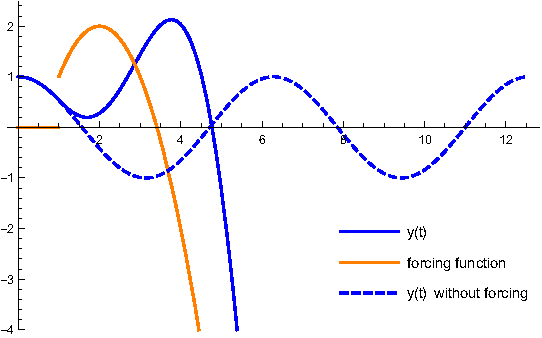
\includegraphics[width=8.5cm]{images/Heaviside_oscillator.pdf}}
}

\subsection{Impulsive Forcing}

\slide[Imagine hitting a golf ball from rest at $t=c$]{\vspace{-1em}

\tikz{\draw (0,0) node{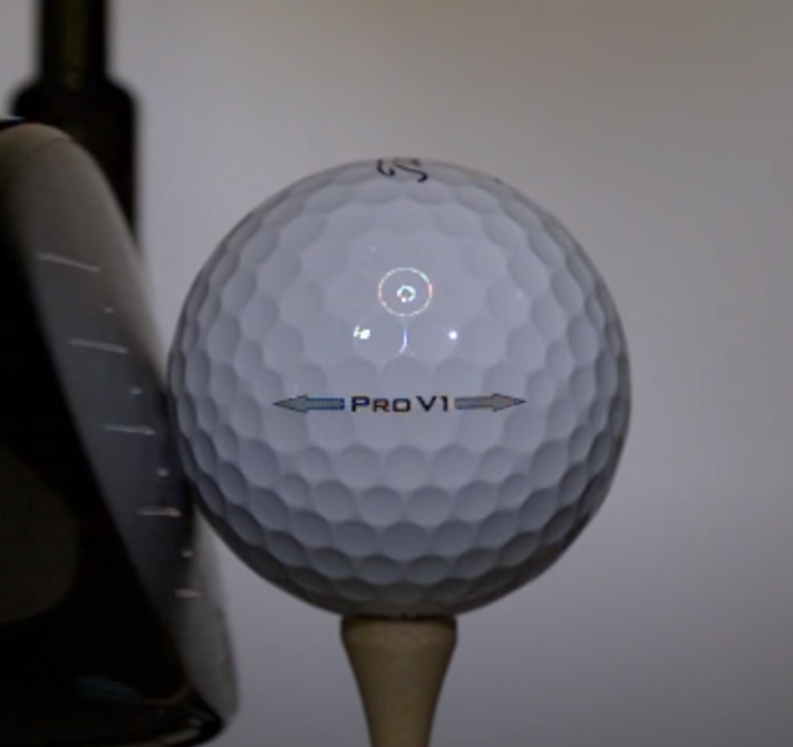
\includegraphics[height=.175\linewidth]{images/golf_ball_1.png}}; \draw[black] (0,-.1) node[fill=white, fill opacity=0.75, text opacity=1, outer sep=0.01, inner sep=1]{\scriptsize$v(0^-)=0$}; }\hfill \tikz{\draw (0,0) node{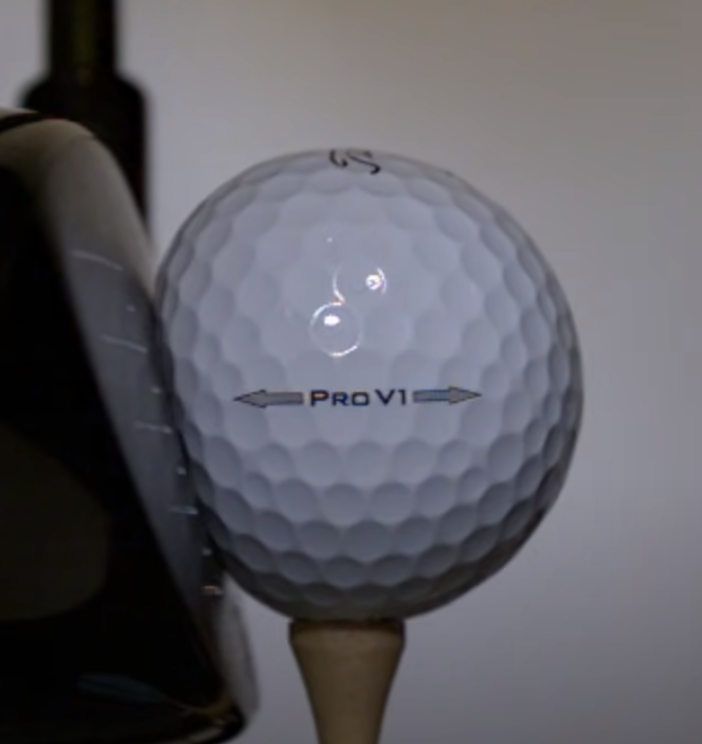
\includegraphics[height=.175\linewidth]{images/golf_ball_2.png}}} \hfill \tikz{\draw (0,0) node{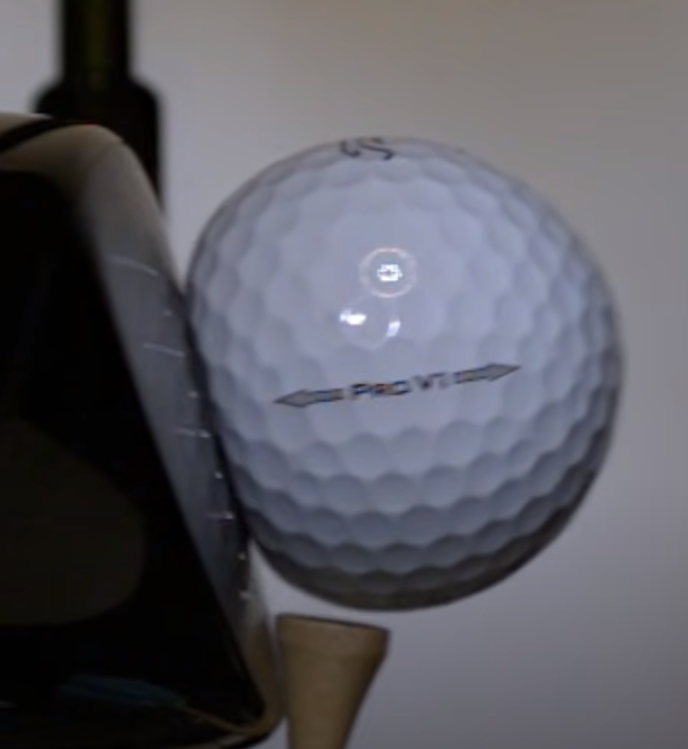
\includegraphics[height=.175\linewidth]{images/golf_ball_3.png}}; } \hfill \tikz{\draw (0,0) node{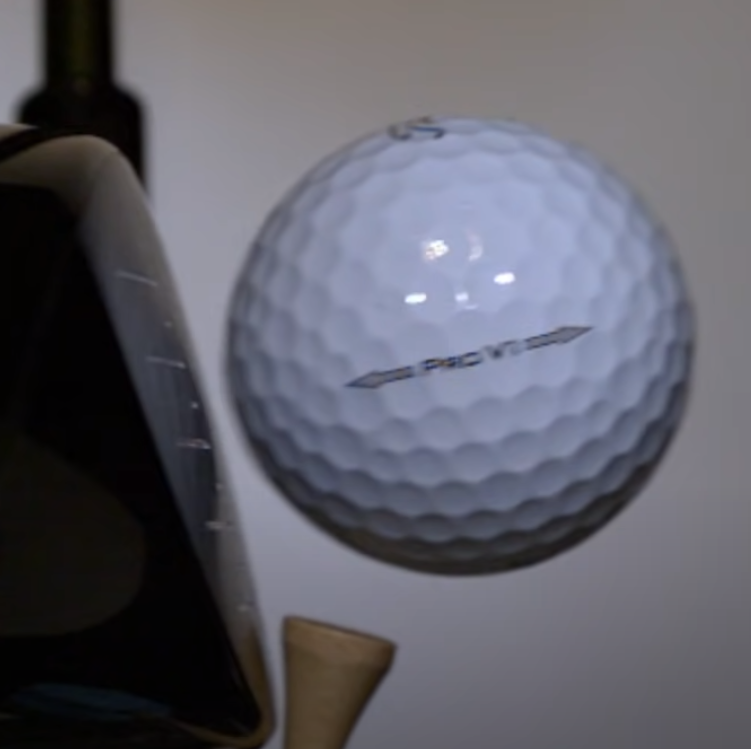
\includegraphics[height=.175\linewidth]{images/golf_ball_4.png}}; \draw[black] (.3,.1) node[fill=white, fill opacity=0.75, text opacity=1, outer sep=0.01, inner sep=1, rotate=30]{\scriptsize$v(0^+)\gg0$}; }

\tiny source:  \url{https://www.youtube.com/watch?v=6TA1s1oNpbk&t=80s}
\normalsize\vspace{-1em}

\twomini[.6]{.6}{.33}{
 \vspace{1.5em}
Suddenly a large force is applied to the ball for a very brief period of time.

\vspace{0.75em}
\student{\uline{Idea:} Describe the force as $\frac{d}{dt}u(t-c)$.

\vspace{1em}

\begin{tikzpicture}[xscale=2, yscale=2]
 \draw[] (0,0)--(0.5,0)--(0.5,0.3)--(1,0.3); 
 \draw[] (-.15,0) node{\tiny 0}; 
 \draw[] (-.15,0.3) node{\tiny 1}; 
 \draw[] (0.5,-.15) node{\tiny t=c};
 


  \draw[->] (1.1,0.00)  to [out=-30,in=-150] (1.45,0.00) node[below, xshift=-0.8em]{$ \small \frac{d}{dt}$}; 
  \draw[<-] (1.1,0.25)  to [out=30,in=150] (1.45,0.25) node[above, xshift=-0.8em]{$ \small\intop$}; 
  
  \draw[] (1.75,0)--(2.75,0); 
  \draw[->] (2.25,0)--(2.25,0.5)node[yshift=.3em]{$\infty$}; 
   \draw[] (1.6,0) node{\tiny 0}; 
 \draw[] (2.25,-.15) node{\tiny t=c};
\draw[] (3,0.35) node[align=center, draw, thin]{\footnotesize Dirac delta\\ \footnotesize function}; 
 \end{tikzpicture}

}
}{
\tikzplot[\xcoord{1}{$t=c$} ]{2}{2}{.3}{3.5}{t}{\text{force}(t)}{

\foreach \xtau in { .08}{
\draw[ultra thick] (1-\xtau,0)--(-8,0) ;
\draw[ultra thick] (1-\xtau, 0.25/\xtau)--(1+\xtau,0.25/\xtau) ;
\draw[thick, dashed] (1-\xtau,0.25/\xtau)--(1-\xtau,0) ;
\draw[thick, dashed] (1+\xtau,0.25/\xtau)--(1+\xtau,0) ;
\draw[ultra thick] (1+\xtau,0)--(6,0) ;

}
}
}\vfill
\student{\centerline{Not a well-defined function, but has a well-defined integral. }}
}



\subsection{Dirac Delta}


\slide[Delta Dirac Function: $\delta(t-c) =\frac{d}{dt} u(t-c)$]{\vspace{-0.75em}
\textbf{Theorem:} For any function $f(t)$ that is integrable in some neighbourhood around $c$\[\int_{-\infty}^{\infty} \delta(t-c) f(t) dt = f(c)\]
Integrating a function $f(t)$ against $\delta(t-c)$ essentially "selects" the value of  $f(t)$ at $t=c$
\vfill

More generally
\twomini[.25]{.65}{.35}{
\[\int_a^b \delta(t-c)f(t) dt =\student{ \begin{cases} f(c)& a\leq c\leq b  \\ 0&\text{otherwise}\end{cases}}\]
}{


\tikzplot[\xcoord{0.8}{c}\xcoord{-0.5}{a}, \xcoord{1.5}{b} ]{1.8}{2.2}{.7}{2}{t}{}{

\foreach \xtau in { .01}{
\draw[ultra thick] (0.8-\xtau,0)--(-8,0) ;
\draw[ultra thick] (0.8-\xtau, 0.3/\xtau)--(1+\xtau,0.3/\xtau) ;
\draw[] (0.8-\xtau,0.25/\xtau)--(0.8-\xtau,0) ;
\draw[] (0.8+\xtau,0.25/\xtau)--(0.8+\xtau,0) ;
\draw[] (1.55,1.7) node{$\delta(t-c)$};
\draw[ultra thick] (0.8+\xtau,0)--(6,0) ;
\draw[black, ultra thick, domain=-2:2.2] plot (\x,0.9*\x^2-0.45*\x^3) node[right, above, xshift=-1em, yshift=2em]{$f(t)$};

}
}


}
}

\slide[Sketch of ``proof'':]{
Approximate the Dirac delta function as normalized pulse:\[ \text{Let }\delta_\tau =  \frac{u(t+\tau)-u(t-\tau)}{2\tau}, \text{and use the approximation  }\delta(t)\approx \lim_{\tau \to 0} \delta_\tau(t)\]
\algn{\int_{-\infty}^{\infty}\delta(t-c)f(t) dt &= \int_{-\infty}^{\infty} \left( \lim_{\tau \to 0} \delta_{\tau}(t-c)\right) f(t) dt\\
&=\lim_{\tau \to 0}  \int_{-\infty}^{\infty}  \delta_{\tau}(t-c) f(t) dt\\
&=\lim_{\tau \to 0}  \frac{1}{2\tau}\int_{c-\tau}^{c+\tau}f(t)dt\\&=\lim_{\tau \to 0} \frac{F(c+\tau)-F(c-\tau)}{2\tau} =f(c)
}
}

\slide[Laplace transform of $\delta(t)$]{
Integrating a function $f(t)$ against $\delta(t-c)$ essentially "selects" the value of  $f(t)$ at $t=c$\vfill
Assuming $c>0$
\student{
\algn{\ucover{\lap{\delta(t-c)}=} & \lapint{\delta(t-c) }\\
=&\int_{-\infty}^{\infty} e^{-st} \delta(t-c) dt =e^{-sc}}
}
Special case: $c=0$
\student{\algn{\ucover{\lap{\delta(t)}=\lim_{c \to 0^+}  \lap{\delta(t-c)}} =  \lim_{c \to 0^+}  e^{-sc} = 1 }}

}
\subsection{Example}

\slide[Solve: \hfill $y\pp+6y\p+45y=6\delta(t-5)$ \hfill with $\larray{y(0)=1\\y\p(0)=0}$]{\vspace{-2em}\student{
\algn{
 (s^2+6s+45)Y(s)-(6+s)&= 6e^{-5s} \quad \Rightarrow \quad Y(s) =\frac{6e^{-5s}+s+6}{s^2+6s+45} \\\\
 Y(s)= e^{-5s}\underbrace{\frac{6}{(s+3)^2+36}}_{\lap{e^{-3t}\sin(6t)}} &+ \underbrace{\frac{s+3}{(s+3)^2+36}}_{\lap{e^{-3t}\cos(6t)}} + \frac{3}{(s+3)^2+36} \\\\
y(t) = \left[ e^{-3t}\sin(6t)\right]_{t=t-5} &+ e^{-3t}\paren{\cos(6t) + \frac12 \sin(6t) }\\
= e^{-3(t-5)}\sin(6(t-5)) &+  e^{-3t}\paren{\cos(6t) + \frac12 \sin(6t) }
}  
}
}

\slide[]{
\[y(t)=e^{-3(t-5)}\sin(6(t-5)) +  e^{-3t}\paren{\cos(6t) + \frac12 \sin(6t) }\]
\vfill
\centerline{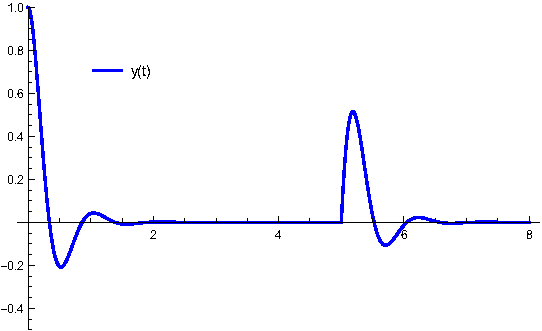
\includegraphics[width=8.5cm]{images/Dirac_overdamped.pdf}}
}


\begin{comment}
\subsection{Convolution Theorem}
\slide[Products in Laplace Space]{\vspace{-1em}
The second shift theorem is a special case of a product in Laplace space\[\lap{f(t-c)u(t-c)} = \underbrace{e^{-sc}}_{G(s)}F(s)\]\vfill
Inversion of the general case requires the use of a convolution
\[\lapinv{F(s) G(s) } = (f * g)(t) = \intop_0^t f(\tau)g(t-\tau) d\tau\] 
\ex{$\lapinv{\frac{e^{-3s}}{s} \frac{2}{s^2} }$ \student{Note:  $\lapinv{e^{-3s}\frac{2}{s^3}}=u(t-3)(t-3)^2$}}
\student{\algn{&=\intop_0^t u(\tau-3) 2(t-\tau) d \tau =\begin{cases} 0&t<3 \\ \intop_3^t 2(t-\tau) d \tau  & t>3 \end{cases} \\
&=\begin{cases} 0&t<3 \\  \left[2t\tau-\tau^2\right]_{\tau=3}^{t} & t>3 \end{cases}  =  u(t-3) (t-3)^2
}}
}
\slide{\ex{$y\p+6y=u(t-1)\student{=\begin{cases}
0 & t<1\\
1 & t\geq1
\end{cases}}$ \hspace{1.5em} with $\larray{y(0)=y_0\\y'(0)=v_0}$}
\student{\twomini[.55]{.6}{.3}{\algn{ sY-&y_0+6Y=\frac{e^{-s}}{s}\\
Y&=\frac{\frac{e^{-s}}{s}+y_0}{s+6}=\frac{e^{-s}}{s(s+6)}+\frac{y_0}{s+6}\\
Y(s)&=\frac{1}{6}\frac{e^{-s}}{s}-\frac{1}{6}\frac{e^{-s}}{s+6}+\frac{y_0}{s+6}\\
& \downarrow \mathcal{L}^{-1}\\
y(t)&=\frac16 u(t-1)-\frac16 e^{-6(t-1)} u(t-1)+y_0e^{-6t}
}\vfill}{$\frac{1}{s(s+6)}=\frac{A}{s}+\frac{B}{s+6}$\\~\\$\Rightarrow 1=A(s+6)+Bs $\\~\\$\Rightarrow \arr{l}{1=6A\\0=A+B}$ \\~\\$\Rightarrow \arr{l}{A=\frac16\\B=-\frac16}$ \vfill}}
\tikzplot[
\student{\xcoord{3}{1} \ycoord{1.25}{\frac16}}
]{.1}{10}{.1}{1.5}{t}{y(t)}{
\student{
\draw[domain=0:2, thick, samples=100] plot ({\x*1.5}, {.8*exp(-\x)});
\draw[domain=2:10, thick, samples=100] plot ({\x*1.5}, {.8*exp(-\x)+(1-exp(-(\x-2)))*1.25});
\draw[domain=0:10, thick, dashed, samples=100] plot ({\x*1.5}, {1.25});
}}
}



\slide{\ex{$y\pp+2y\p+5y=u(t-5)-u(t-15)$, \quad $y(0)=0.1$, $y\p(0)=0$}
\student{
\algn{s^2Y(s)-&0.1s+2sY(s)-0.2+5Y(s)=\frac{e^{-5s}}{s} - \frac{e^{-15s}}{s}\\
Y(s)&= \frac{  \paren{\frac{e^{-s}}{s} - \frac{e^{-2s}}{s}} + 0.1s+0.2}{s^2+2s+5}\\
&=  \paren{ e^{-5s} - e^{-15s}}  \underbrace{\frac{ 1}{s(s^2+2s+5)}}_{F(s)}+   \underbrace{\frac{ 0.1s +0.2}{s^2+2s+5}}_{\text{homogeneous part}}\\
s^2+2s+5 &= (s+1)^2+4 \Rightarrow\text{homog. part} = \underbrace{\frac{0.1s}{ (s+1)^2+4}}_{\text{exp} \cdot \cos}  + \underbrace{\frac{0.2}{ (s+1)^2+4}}_{\text{exp} \cdot \sin}
\\\\
y(t)&=u(t-5)\left[ \lapinv{F(s)} \right]_{t=t-5}\\
&\phantom{=} - u(t-15)\left[ \lapinv{F(s)} \right]_{t=t-15}\\
&\phantom{=} + 0.1e^{-t}\cos(2t)+0.1 e^{-t}\sin(2t)
}
}
}%end slide

\settoggle{covered}{false}
\slide{$\lapinv{\frac{1}{s(s^2+2s+5)}}=\;???$ 

\student{
\algn{F(s)=\frac{1}{s(s^2+2s+5)} & = \frac{A}{s} +\frac{Bs+C}{s^2+2s+5}\\
1&=As^2+2As+5A + Bs^2+Cs\\
\text{constant terms: } 1&= 5A \qquad \Rightarrow A=\frac15 \\
\text{$s$ terms: } 0 &= 2A+C   \qquad \Rightarrow C=-2A=-\frac25\\
\text{$s^2$ terms: } 0 &=	A+B  \qquad \Rightarrow B=-A=-\frac15\\
F(s) &= \frac{1}{5s} - \frac15 \frac{s+2}{(s+1)^2+2^2}\\
&=  \frac{1}{5s} -  \frac15 \paren{\frac{s+1}{(s+1)^2+2^2}  - \frac{1}{(s+1)^2+2^2}}  \\
f(t) &= \frac15 \paren{1-e^{-t}\paren{cos(2t) -\frac12 \sin(2t)}}}
}
}

\slide{\vspace{-2em}
\algn{y(t)&=u(t-5)\frac15 \paren{1-e^{-(t-5)}\paren{cos(2(t-5)) -\frac12 \sin(2(t-5))}}\\
&\phantom{=} - u(t-15)\frac15 \paren{1-e^{-(t-15)}\paren{cos(2(t-15)) -\frac12 \sin(2(t-15))}}\\\
&\phantom{=} + 0.1e^{-t}(\cos(2t)+\sin(2t))}

\vspace{1em}
\centerline{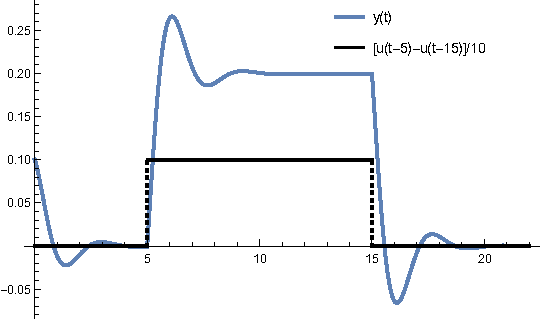
\includegraphics[width=8.5cm]{images/Heaviside_jiggle.pdf}}
}
\end{comment}

\end{document}